%! TeX program = pdflatex
%! TeX TS-program = pdflatex

\documentclass[10pt]{IEEEtran}
\usepackage{amsmath}
\usepackage[utf8]{inputenc}
\usepackage{fontenc}
\usepackage{dirtytalk}
\usepackage[dvipsnames]{xcolor}
\usepackage{tikz}
\usepackage{varwidth}
\usepackage{csquotes}
\usepackage{listings}
\usepackage{graphicx}
\usepackage[spanish]{babel}
\usetikzlibrary{positioning}
\usepackage{biblatex}
\addbibresource{bibl.bib}
\tikzset{
  x=1em,
  y=1em,
}
\lstset{
  basicstyle=\ttfamily\footnotesize,
  showstringspaces=false,
  commentstyle=\itshape,
  keywordstyle=\bfseries\color{cyan},
  stringstyle=\ttfamily,
  language=C,
  tabsize=2,
  breaklines=true,
  breakatwhitespace=true,
  escapeinside={\%*}{*)},
  morekeywords={
    cv,
    filter2D,
    abs,
    NORM_MINMAX,
    CV_8UC1,
    THRESH_BINARY,
    threshold,
    Point,
    BORDER_DEFAULT,
    normalize,
    equalizeHist
  },
}

\graphicspath{{code/res/}}

\title{Transferencia de color y recuperación de color de una imagen}

\author{ Brandon Marquez Salazar }

\begin{document}
  \maketitle
  \section{Introducción}
  La transferencia de color es una técnica utilizada en el procesamiento de imágenes para mejorar
  la calidad de la imagen, así mismo, es posible ver una posible aplicación en la Astrofotografía,
  la Microscopía, la Mercadotecnia, la Fotografía, entre otras áreas donde la visualización de la imagen es importante.

  \section{Materiales y métodos}
  El programa se realizará utilizando el lenguaje C++ y la biblioteca OpenCV para la manipulación de gráficos.
  El algoritmo de transferencia de color utilizado fue desarrollado en \cite{Reinhard2001}.
  Se utilizará una imagen y su contraparte en escala de grises.

  \section{Objetivos}
  Se proponen dos hipótesis.
  La primera hipótesis supone que el color de la imagen regresará de manera similar al color original.
  La segunda hipótesis supone que el color de la imagen considerará algún promediado repartido sobre el relieve de la escala de grises.

  \section{Procedimiento}
  Se utilizó el programa en C++ con la biblioteca OpenCV para la manipulación de gráficos, a fin de
  tomar la imagen en escala de grises como \textit{input} y su contraparte original como \textit{source}.

  \section{Resultados}
  La imagen resultante del proceso obtuvo un promediado del color de la imagen original repartido
  sobre el relieve de la escala de grises.

    \begin{figure}[ht]
      \centering
      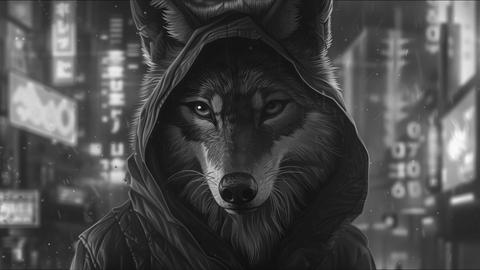
\includegraphics[width=0.8\linewidth]{res/Original.png}
      \caption{Imagen de entrada}
    \end{figure}

    \begin{figure}[ht]
      \centering
      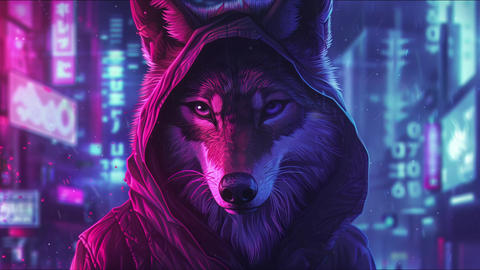
\includegraphics[width=0.8\linewidth]{res/Reference.png}
      \caption{Imagen de referencia}
    \end{figure}

    \begin{figure}[ht]
      \centering
      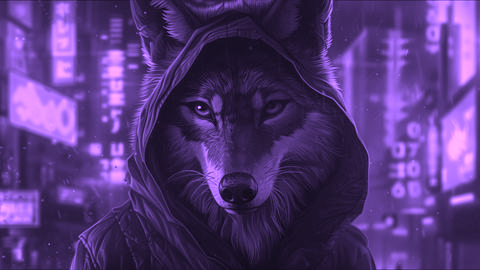
\includegraphics[width=0.8\linewidth]{res/Transfer.png}
      \caption{Imagen resultante}
    \end{figure}

  \section{Conclusiones}
  Este experimento demostró que la recuperación de color es un proceso más complejo. Se puede deducir que la
  razón de que el resultado tuviera este comportamiento, se debe a que el proceso propuesto en \cite{Reinhard2001},
  utiliza la media y la desviación estándar de la imagen source.

  \printbibliography
\end{document}
